% W2 / AC-3.* — vibrato spectrograms, hear panel, WT diversity gallery
% Included from main.tex (separate file to reduce merge risk with T2/T3 Methods edits).

\subsection{Vibrato playback and spectrograms}
\label{sec:vibrato-eval}

RQ: do wrap-seam differences remain visible under \emph{dynamic} pitch (slow vibrato), not only static tiled periods?
Figure~\ref{fig:vibrato-spectrogram} renders the same holdout cracked period, DualCosine bake, and refit \textbf{Ours (hybrid GA--PPO)} champion under shared sinusoidal vibrato ($\pm 3\%$ depth at $5$\,Hz around $220$\,Hz).
Panels (a--c) show magnitude spectrograms; (d--e) show DualCosine$-$no-bake and Ours$-$no-bake differences; (g) reports cycle-local prolonged $R$ alongside a modulated-playback residual under the same pitch envelope.
On the annotated high-wrap tile, Ours retains high cycle $R$ and high modulated $R$, while DualCosine remains the weakest classical comparator.
This is objective spectrogram / residual evidence only---not a formal listening study.
Source: \texttt{reelsynth/scripts/bench\_vibrato\_spectrogram.py}; artifacts under \texttt{brand/artifacts/vibrato\_spectrogram/}.

\begin{figure*}[t]
  \centering
  
\includegraphics[width=\textwidth]{figures/fig_vibrato_spectrogram.png}
  \caption{Slow-vibrato spectrogram eval on a high-wrap holdout tile (seed~\texttt{20260719}).
    (a--c)~Magnitude spectrograms for no-bake, DualCosine, and Ours.
    (d--e)~Spectrogram differences vs no-bake.
    (f)~Short waveform excerpt.
    (g)~Absolute $R$: cycle-local prolonged residual, modulated-playback residual on the same tile, and mean modulated $R$ over top-wrap tiles.
    Accessibility: Okabe--Ito hues; difference maps use diverging coolwarm.
    Formal human A/B scores are out of scope.}
  \label{fig:vibrato-spectrogram}
\end{figure*}

\subsection{Downloadable hear samples}
\label{sec:hear-samples}

As an audible companion to Figure~\ref{fig:meta-heal-samples}, we release five fixed-pitch (A4, $3$\,s, $44.1$\,kHz mono) wavetable clips for no-bake, DualCosine, and Ours-healed periods from the matched-suite holdout
(\texttt{reelsynth/brand/artifacts/meta\_approach\_compare/hear\_samples/}; rebuild via \texttt{scripts/export\_meta\_hear\_samples.py}).
Figure~\ref{fig:hear-samples-panel} shows short waveform excerpts from those WAVs with per-clip absolute $R$.
Readers can download and listen; we do \emph{not} report formal MOS/MUSHRA or claimed A/B listening scores.

\begin{figure*}[t]
  \centering
  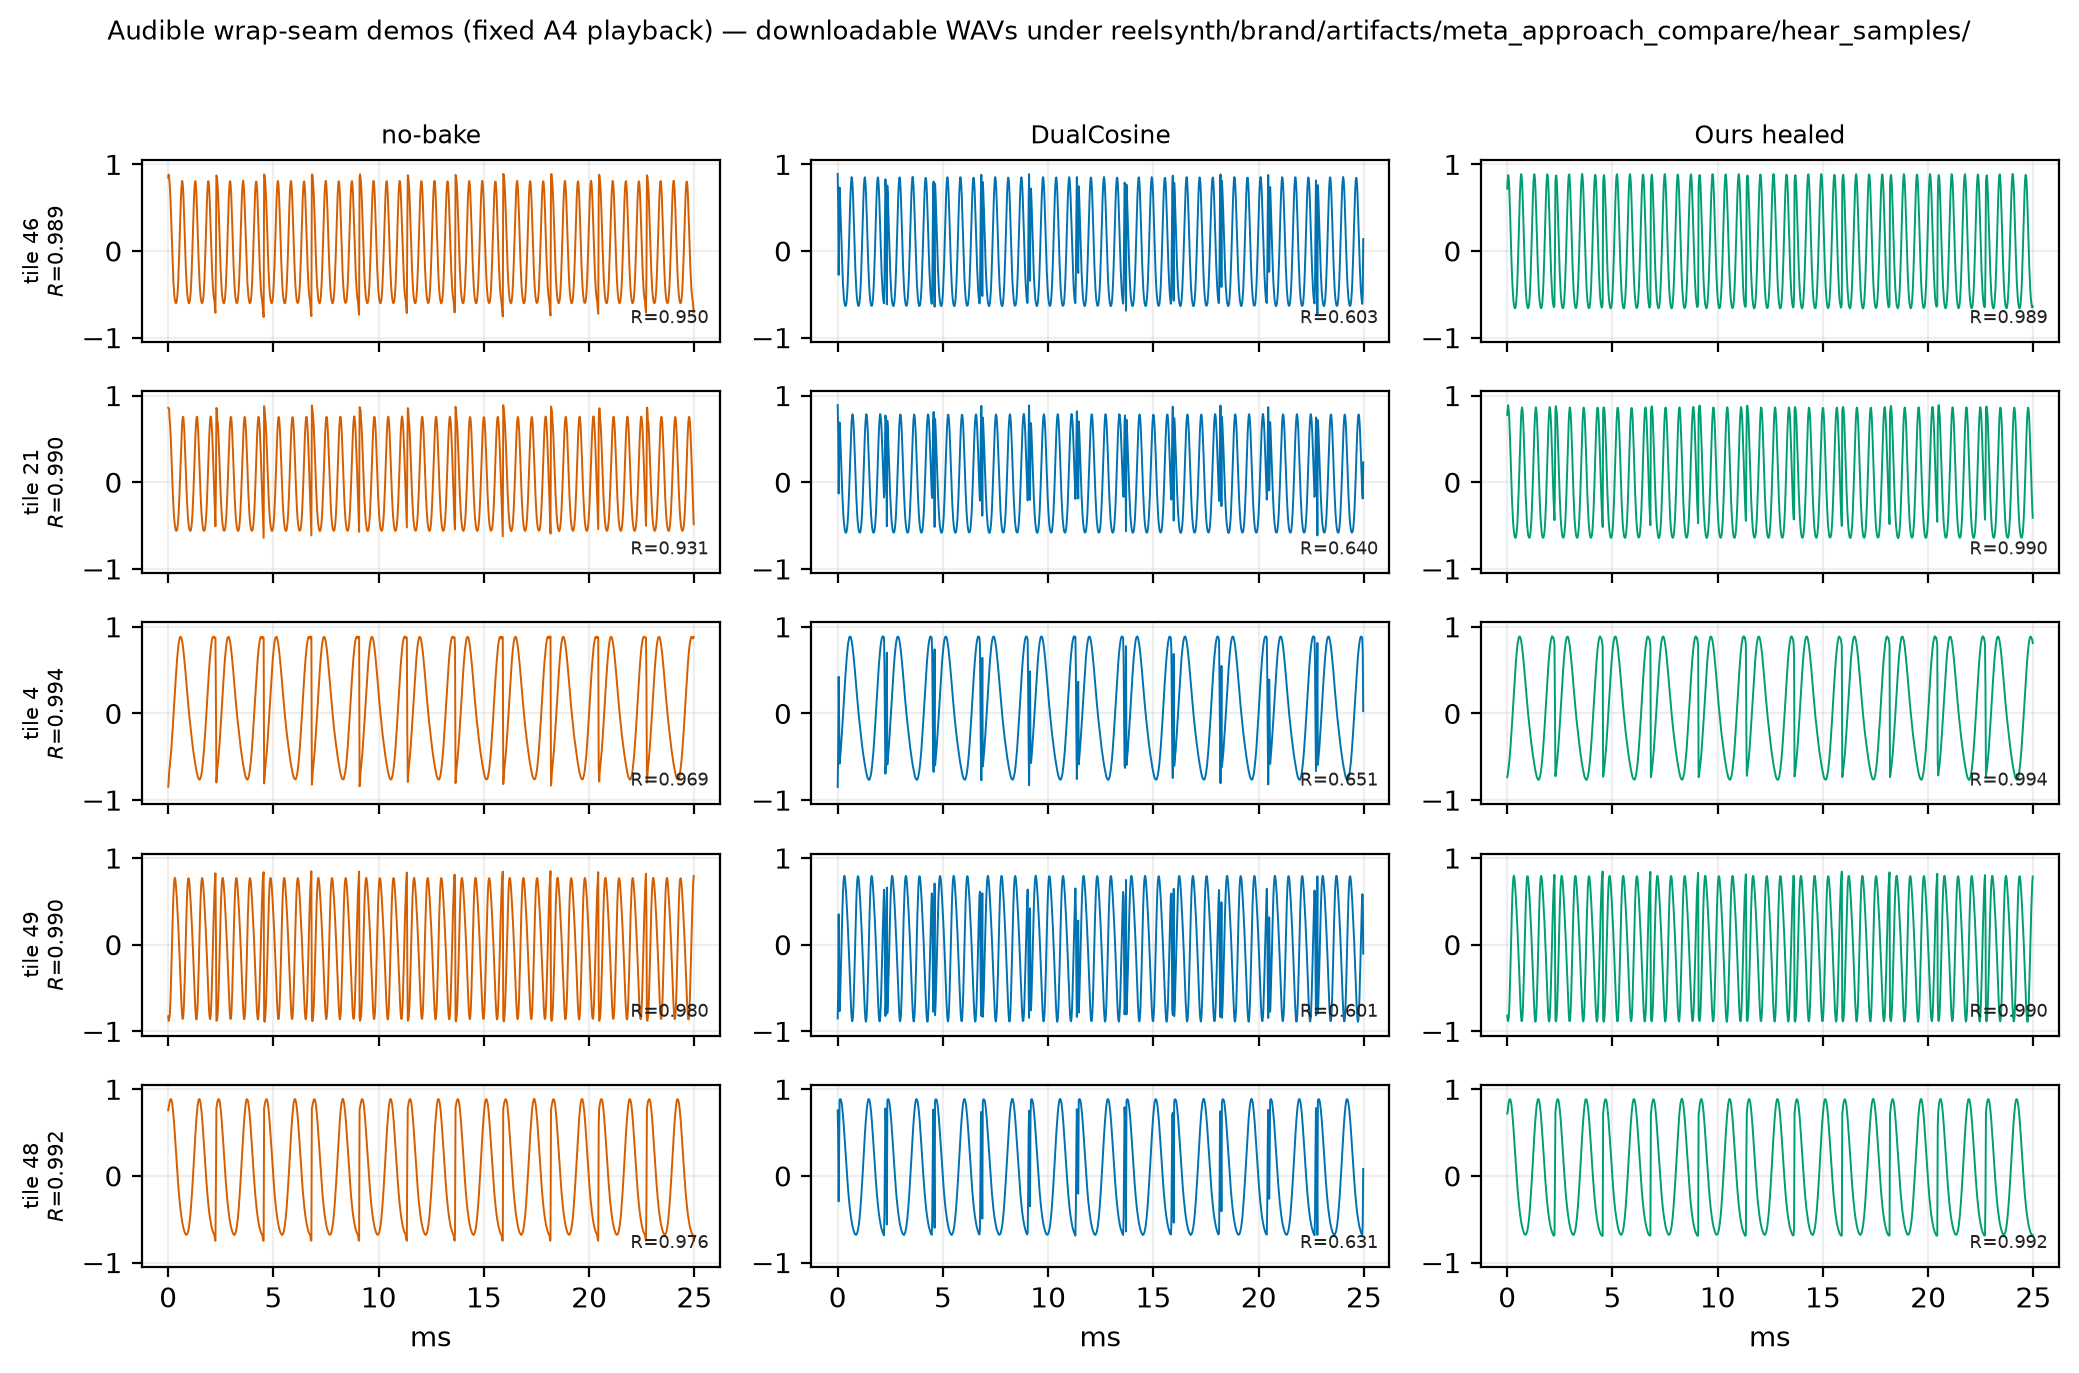
\includegraphics[width=\textwidth]{figures/fig_hear_samples_panel.png}
  \caption{Hear-sample panel from downloadable WAVs under
    \texttt{brand/artifacts/meta\_approach\_compare/hear\_samples/}
    (five holdout tiles; no-bake / DualCosine / Ours).
    Waveforms show the first $\approx 25$\,ms of each clip; $R$ annotations are cycle-local prolonged residuals vs the ideal sibling.
    Not a formal listening study.}
  \label{fig:hear-samples-panel}
\end{figure*}

\subsection{Compact wavetable diversity gallery}
\label{sec:wt-gallery}

Beyond the synthetic sine{+}cliff narrative, Figure~\ref{fig:wt-diversity-gallery} shows a compact gallery of true ReelSynth-exported factory periods (one mid-morph frame per bank) and Adventure Kid Waveforms (AKWF) CC0 single-cycle files already used by the wrap protocol.
Scored means remain in Table~\ref{tab:real-wt} / \texttt{real\_wt\_matrix.json}; this panel is diversity evidence only.
No new NAS was run for the gallery.

\begin{figure*}[t]
  \centering
  
\includegraphics[width=\textwidth]{figures/fig_wt_diversity_gallery.png}
  \caption{Compact wavetable diversity gallery from existing exports (ReelSynth factory banks, top; AKWF CC0 cycles, bottom).
    Mid-morph frames per bank; no new meta-search.
    Quantitative wrap scores: Table~\ref{tab:real-wt}.}
  \label{fig:wt-diversity-gallery}
\end{figure*}
